\documentclass{article}
\usepackage{graphicx}
\usepackage{url}
\usepackage{amssymb}
\usepackage{amsmath}
\usepackage{fullpage}

\newcommand{\R}{{\sf R}}
\newcommand{\code}[1]{\texttt{#1}}
\title{Template}
\author{SC Walker}

\newcounter{exercise}
\numberwithin{exercise}{section}
\newcommand{\exnumber}{\addtocounter{exercise}{1} \theexercise \thinspace}

\usepackage{Sweave}
\begin{document}


\begin{Schunk}
\begin{Sinput}
> library(multitable)
> library(lattice)
> library(tensor)
> library(MASS)
\end{Sinput}
\end{Schunk}

\newpage


\begin{Schunk}
\begin{Sinput}
> ab
\end{Sinput}
\begin{Soutput}
       sppA  sppB  sppC
siteA  1.17 -0.04  0.85
siteB  0.65 -0.06 -0.37
siteC  0.51 -2.73  1.07
siteD -1.19  2.81  0.17
siteE -0.69 -0.21  0.38
\end{Soutput}
\end{Schunk}

\newpage

\begin{Schunk}
\begin{Sinput}
> tp
\end{Sinput}
\begin{Soutput}
siteA siteB siteC siteD siteE 
-1.04  0.77  0.82 -0.38 -0.06 
\end{Soutput}
\end{Schunk}

\newpage

\begin{Schunk}
\begin{Sinput}
> bs
\end{Sinput}
\begin{Soutput}
 sppA  sppB  sppC 
-0.45 -0.07  1.48 
\end{Soutput}
\end{Schunk}

\newpage

\begin{Schunk}
\begin{Sinput}
> dl <- data.list(abundance = ab, temperature = tp, bodysize = bs, dnames = c("sites", 
+     "species"))
> dl
\end{Sinput}
\begin{Soutput}
abundance:
---------
       sppA  sppB  sppC
siteA  1.17 -0.04  0.85
siteB  0.65 -0.06 -0.37
siteC  0.51 -2.73  1.07
siteD -1.19  2.81  0.17
siteE -0.69 -0.21  0.38
Replicated along:  || sites || species || 


temperature:
-----------
siteA siteB siteC siteD siteE 
-1.04  0.77  0.82 -0.38 -0.06 
Replicated along:  || sites || 


bodysize:
--------
 sppA  sppB  sppC 
-0.45 -0.07  1.48 
Replicated along:  || species || 


REPLICATION DIMENSIONS: 
  sites species 
      5       3 
\end{Soutput}
\end{Schunk}

\newpage

\begin{Schunk}
\begin{Sinput}
> summary(dl)
\end{Sinput}
\begin{Soutput}
$dims
        abundance temperature bodysize
sites        TRUE        TRUE    FALSE
species      TRUE       FALSE     TRUE

$modes
  abundance temperature    bodysize 
  "numeric"   "numeric"   "numeric" 
\end{Soutput}
\end{Schunk}

\newpage

\begin{Schunk}
\begin{Sinput}
> str(dl)
\end{Sinput}
\begin{Soutput}
List of 3
 $ abundance  : num [1:5, 1:3] 1.17 0.65 0.51 -1.19 -0.69 -0.04 -0.06 -2.73 2.81 -0.21 ...
 $ temperature: num [1:5(1d)] -1.04 0.77 0.82 -0.38 -0.06
 $ bodysize   : num [1:3(1d)] -0.45 -0.07 1.48
\end{Soutput}
\end{Schunk}

\newpage

\begin{Schunk}
\begin{Sinput}
> dl[1:3, ]
\end{Sinput}
\begin{Soutput}
abundance:
---------
      sppA  sppB  sppC
siteA 1.17 -0.04  0.85
siteB 0.65 -0.06 -0.37
siteC 0.51 -2.73  1.07
Replicated along:  || sites || species || 


temperature:
-----------
siteA siteB siteC 
-1.04  0.77  0.82 
Replicated along:  || sites || 


bodysize:
--------
 sppA  sppB  sppC 
-0.45 -0.07  1.48 
Replicated along:  || species || 


REPLICATION DIMENSIONS: 
  sites species 
      3       3 
\end{Soutput}
\end{Schunk}

\newpage

\begin{Schunk}
\begin{Sinput}
> dl[, "sppB"]
\end{Sinput}
\begin{Soutput}
abundance:
---------
       sppB
siteA -0.04
siteB -0.06
siteC -2.73
siteD  2.81
siteE -0.21
Replicated along:  || sites || species || 


temperature:
-----------
siteA siteB siteC siteD siteE 
-1.04  0.77  0.82 -0.38 -0.06 
Replicated along:  || sites || 


bodysize:
--------
 sppB 
-0.07 
Replicated along:  || species || 


REPLICATION DIMENSIONS: 
  sites species 
      5       1 
\end{Soutput}
\end{Schunk}

\newpage

\begin{Schunk}
\begin{Sinput}
> dl$temperature <- scale(dl$temperature)
> dl
\end{Sinput}
\begin{Soutput}
abundance:
---------
       sppA  sppB  sppC
siteA  1.17 -0.04  0.85
siteB  0.65 -0.06 -0.37
siteC  0.51 -2.73  1.07
siteD -1.19  2.81  0.17
siteE -0.69 -0.21  0.38
Replicated along:  || sites || species || 


temperature:
-----------
     siteA      siteB      siteC      siteD      siteE 
-1.3453605  0.9475797  1.0109206 -0.5092608 -0.1038791 
attr(,"scaled:center")
[1] 0.022
attr(,"scaled:scale")
[1] 0.7893795
Replicated along:  || sites || 


bodysize:
--------
 sppA  sppB  sppC 
-0.45 -0.07  1.48 
Replicated along:  || species || 


REPLICATION DIMENSIONS: 
  sites species 
      5       3 
\end{Soutput}
\end{Schunk}

\newpage

\begin{Schunk}
\begin{Sinput}
> lm(abundance ~ temperature * bodysize, dl)
\end{Sinput}
\begin{Soutput}
Call:
lm(formula = abundance ~ temperature * bodysize, data = dl)

Coefficients:
         (Intercept)           temperature              bodysize  temperature:bodysize  
             0.08795              -0.40439               0.20848               0.09822  
\end{Soutput}
\end{Schunk}

\newpage

\begin{Schunk}
\begin{Sinput}
> rlm(abundance ~ temperature * bodysize, dl)
\end{Sinput}
\begin{Soutput}
Call:
rlm(formula = abundance ~ temperature * bodysize, data = dl)
Converged in 5 iterations

Coefficients:
         (Intercept)          temperature             bodysize temperature:bodysize 
          0.08346409          -0.22734601           0.21060731           0.01419073 

Degrees of freedom: 15 total; 11 residual
Scale estimate: 1.04 
\end{Soutput}
\end{Schunk}

\newpage

\begin{Schunk}
\begin{Sinput}
> plot(abundance ~ temperature, dl)
\end{Sinput}
\end{Schunk}
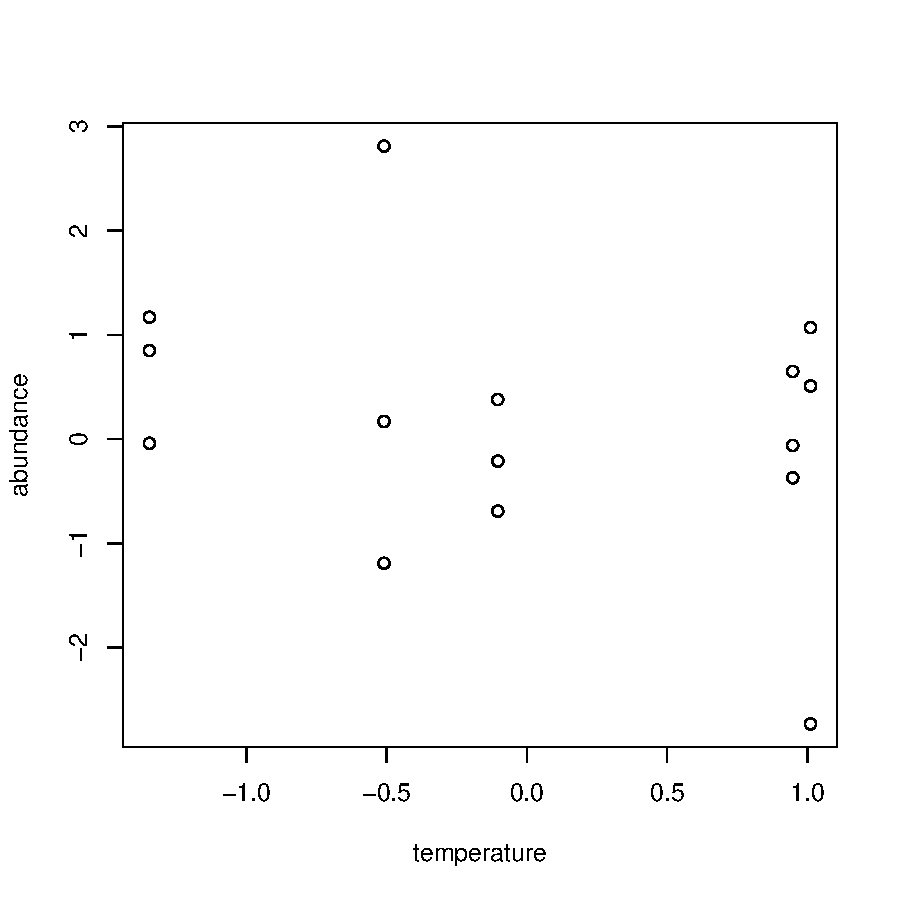
\includegraphics{sweave-015}

\newpage

\begin{Schunk}
\begin{Sinput}
> as.data.frame(dl)
\end{Sinput}
\begin{Soutput}
   abundance temperature bodysize
1       1.17  -1.3453605    -0.45
2       0.65   0.9475797    -0.45
3       0.51   1.0109206    -0.45
4      -1.19  -0.5092608    -0.45
5      -0.69  -0.1038791    -0.45
6      -0.04  -1.3453605    -0.07
7      -0.06   0.9475797    -0.07
8      -2.73   1.0109206    -0.07
9       2.81  -0.5092608    -0.07
10     -0.21  -0.1038791    -0.07
11      0.85  -1.3453605     1.48
12     -0.37   0.9475797     1.48
13      1.07   1.0109206     1.48
14      0.17  -0.5092608     1.48
15      0.38  -0.1038791     1.48
\end{Soutput}
\end{Schunk}

\newpage

\begin{Schunk}
\begin{Sinput}
> variablize(dl)
\end{Sinput}
\begin{Soutput}
      abundance.sppA abundance.sppB abundance.sppC temperature
siteA           1.17          -0.04           0.85  -1.3453605
siteB           0.65          -0.06          -0.37   0.9475797
siteC           0.51          -2.73           1.07   1.0109206
siteD          -1.19           2.81           0.17  -0.5092608
siteE          -0.69          -0.21           0.38  -0.1038791
\end{Soutput}
\end{Schunk}

\newpage

\begin{Schunk}
\begin{Sinput}
> variablize(aperm(dl, c(2, 1)))
\end{Sinput}
\begin{Soutput}
     abundance.siteA abundance.siteB abundance.siteC abundance.siteD abundance.siteE bodysize
sppA            1.17            0.65            0.51           -1.19           -0.69    -0.45
sppB           -0.04           -0.06           -2.73            2.81           -0.21    -0.07
sppC            0.85           -0.37            1.07            0.17            0.38     1.48
\end{Soutput}
\end{Schunk}

\newpage

\begin{Schunk}
\begin{Sinput}
> xyplot(abundance ~ temperature | bodysize, data = as.data.frame(dl))
\end{Sinput}
\end{Schunk}
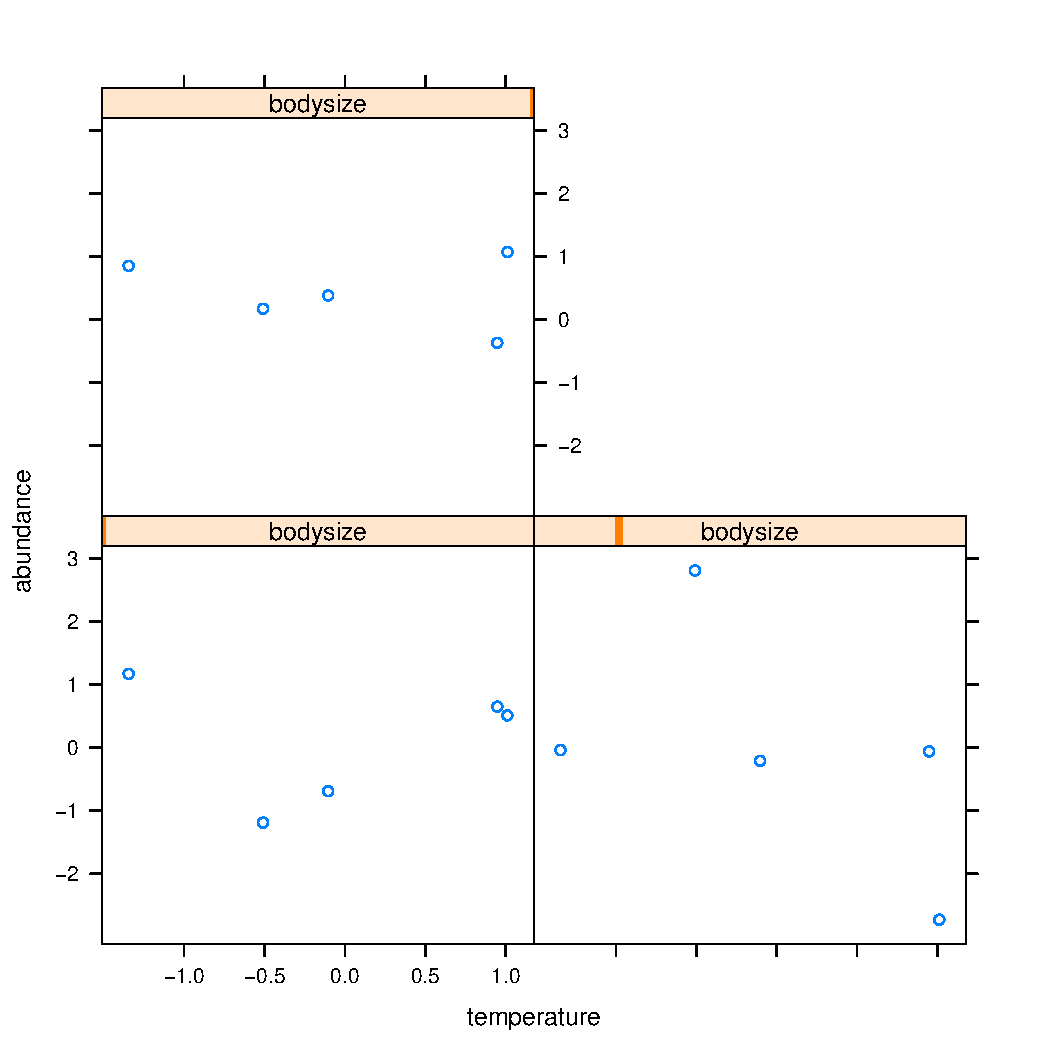
\includegraphics{sweave-019}

\begin{Schunk}
\begin{Soutput}
quartz 
     2 
\end{Soutput}
\end{Schunk}

\newpage


\begin{Schunk}
\begin{Sinput}
> dl <- data.list(Abundance = Y, X, W, Z, dnames = c("time", "species", "basin"))
\end{Sinput}
\end{Schunk}

\newpage

\begin{Schunk}
\begin{Sinput}
> summary(dl)
\end{Sinput}
\begin{Soutput}
$dims
        Abundance Temp.CV..Fluoro. Chl.CV..Fluoro. MaxTemp..Fl. MaxChl..Fl. Depth.TempMax.Fl.
time         TRUE             TRUE            TRUE         TRUE        TRUE              TRUE
species      TRUE            FALSE           FALSE        FALSE       FALSE             FALSE
basin        TRUE             TRUE            TRUE         TRUE        TRUE              TRUE
        DepthChlMax..Fl. Thermocline.Depth  Year  Week Habitat TrophicGroup FeedingType Length
time                TRUE              TRUE  TRUE  TRUE   FALSE        FALSE       FALSE  FALSE
species            FALSE             FALSE FALSE FALSE    TRUE         TRUE        TRUE   TRUE
basin               TRUE              TRUE FALSE FALSE   FALSE        FALSE       FALSE  FALSE
        Predator.protection.
time                   FALSE
species                 TRUE
basin                  FALSE

$modes
           Abundance     Temp.CV..Fluoro.      Chl.CV..Fluoro.         MaxTemp..Fl. 
           "numeric"            "numeric"            "numeric"            "numeric" 
         MaxChl..Fl.    Depth.TempMax.Fl.     DepthChlMax..Fl.    Thermocline.Depth 
           "numeric"            "numeric"            "numeric"            "numeric" 
                Year                 Week              Habitat         TrophicGroup 
           "numeric"            "numeric"            "numeric"            "numeric" 
         FeedingType               Length Predator.protection. 
           "numeric"            "numeric"            "numeric" 
\end{Soutput}
\end{Schunk}

\newpage

\begin{Schunk}
\begin{Sinput}
> str(dl)
\end{Sinput}
\begin{Soutput}
List of 15
 $ Abundance           : num [1:16, 1:12, 1:3] 0.00134 0.00269 0.00361 0.00134 0.00226 ...
 $ Temp.CV..Fluoro.    : num [1:16, 1:3] 0.56 0.52 0.42 0.39 0.41 0.57 0.48 0.48 0.44 0.4 ...
 $ Chl.CV..Fluoro.     : num [1:16, 1:3] 0.92 0.94 1.04 1.05 0.82 0.92 0.79 0.79 0.27 0.27 ...
 $ MaxTemp..Fl.        : num [1:16, 1:3] 23.8 21.1 22.9 26.5 22.8 ...
 $ MaxChl..Fl.         : num [1:16, 1:3] 5.49 4.86 6.21 6.94 7.07 6.82 3.58 6.7 2.43 1.84 ...
 $ Depth.TempMax.Fl.   : num [1:16, 1:3] 0 1 2 0 1 1 0 1 1 0 ...
 $ DepthChlMax..Fl.    : num [1:16, 1:3] 5 4 7 6 5 8 5 6 5 5 ...
 $ Thermocline.Depth   : num [1:16, 1:3] 4.5 4.5 4.5 4.5 4.5 4.5 3.5 3.5 4 4.5 ...
 $ Year                : int [1:16(1d)] 2007 2007 2007 2007 2007 2007 2008 2008 2008 2008 ...
 $ Week                : int [1:16(1d)] 171 185 199 213 227 241 178 188 205 219 ...
 $ Habitat             : factor [1:12(1d)] Pelagic Pelagic Pelagic Pelagic ...
 $ TrophicGroup        : factor [1:12(1d)] Herbivore Herbivore Herbivore Herbivore ...
 $ FeedingType         : factor [1:12(1d)] D-filtration D-filtration B-filtration S-filtration ...
 $ Length              : num [1:12(1d)] 0.96 0.8 0.33 0.77 0.75 1.23 0.18 1.31 0.45 0.36 ...
 $ Predator.protection.: factor [1:12(1d)] N Y N Y ...
\end{Soutput}
\end{Schunk}

\newpage


\begin{Schunk}
\begin{Sinput}
> xyplot(Abundance ~ Chl.CV..Fluoro. | Length, data = as.data.frame(dl))
\end{Sinput}
\end{Schunk}
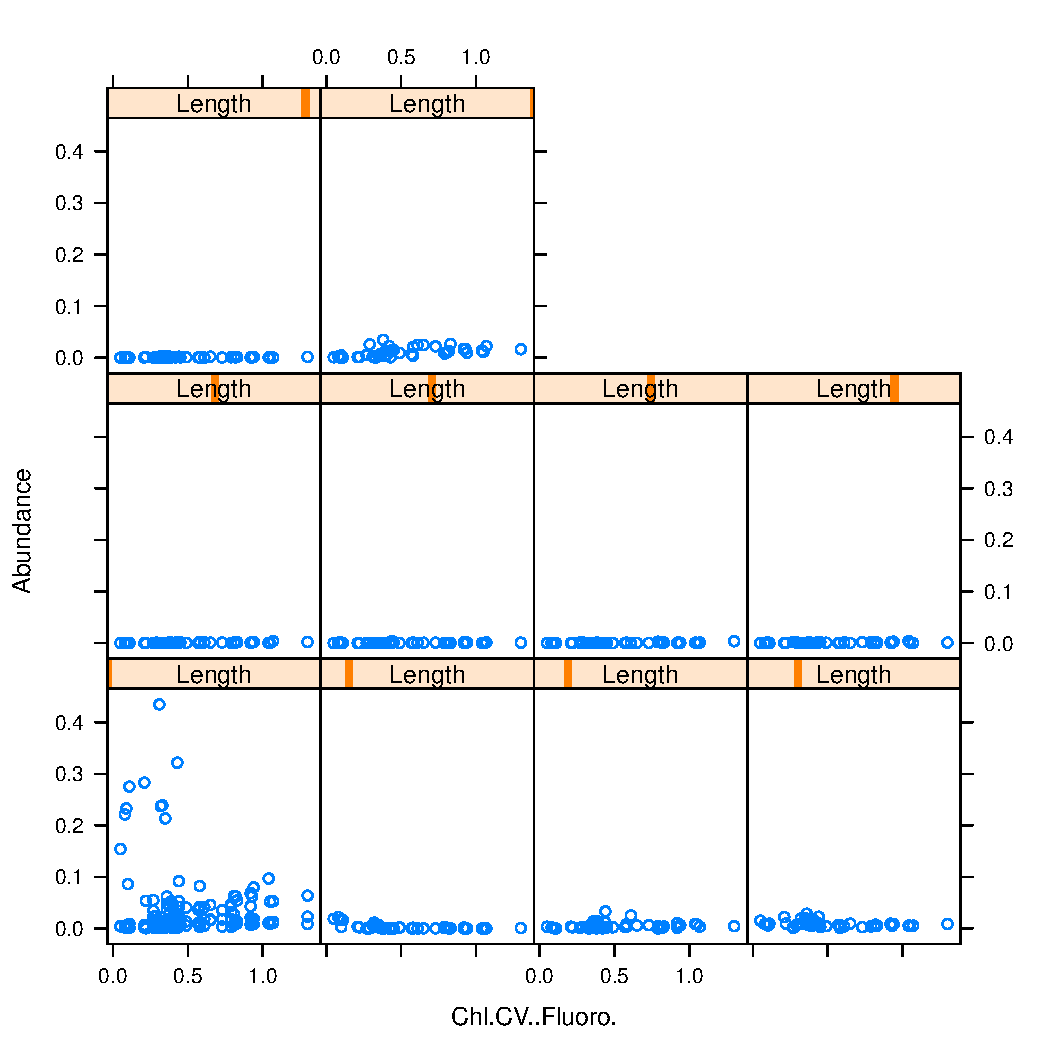
\includegraphics{sweave-026}

\begin{Schunk}
\begin{Sinput}
> pdf("/users/stevenwalker/documents/multitable/multitable/presentations/ESA2011/sweave-026.pdf")
> xyplot(Abundance ~ Chl.CV..Fluoro. | Length, data = as.data.frame(dl))
> dev.off()
\end{Sinput}
\begin{Soutput}
quartz 
     2 
\end{Soutput}
\end{Schunk}

\end{document}
